% !TEX TS-program = pdflatex
% !TEX encoding = UTF-8 Unicode

% This is a simple template for a LaTeX document using the "article" class.
% See "book", "report", "letter" for other types of document.

\documentclass[11pt]{article} % use larger type; default would be 10pt

\usepackage[utf8]{inputenc} % set input encoding (not needed with XeLaTeX)

%%% Examples of Article customizations
% These packages are optional, depending whether you want the features they provide.
% See the LaTeX Companion or other references for full information.

%%% PAGE DIMENSIONS
\usepackage{geometry} % to change the page dimensions
%\geometry{letterpaper} % or letterpaper (US) or a5paper or....
% \geometry{margin=2in} % for example, change the margins to 2 inches all round
% \geometry{landscape} % set up the page for landscape
%   read geometry.pdf for detailed page layout information

\usepackage{graphicx} % support the \includegraphics command and options

% \usepackage[parfill]{parskip} % Activate to begin paragraphs with an empty line rather than an indent

%%% PACKAGES
\usepackage{booktabs} % for much better looking tables
\usepackage{array} % for better arrays (eg matrices) in maths
\usepackage{paralist} % very flexible & customisable lists (eg. enumerate/itemize, etc.)
\usepackage{verbatim} % adds environment for commenting out blocks of text & for better verbatim
\usepackage{subfig} % make it possible to include more than one captioned figure/table in a single float
% These packages are all incorporated in the memoir class to one degree or another...

%%% HEADERS & FOOTERS
\usepackage{fancyhdr} % This should be set AFTER setting up the page geometry
\pagestyle{fancy} % options: empty , plain , fancy
\renewcommand{\headrulewidth}{0pt} % customise the layout...
\lhead{}\chead{}\rhead{}
\lfoot{}\cfoot{\thepage}\rfoot{}

%%% SECTION TITLE APPEARANCE
\usepackage{sectsty}
\allsectionsfont{\sffamily\mdseries\upshape} % (See the fntguide.pdf for font help)
% (This matches ConTeXt defaults)

%%% ToC (table of contents) APPEARANCE
\usepackage[nottoc,notlof,notlot]{tocbibind} % Put the bibliography in the ToC
\usepackage[titles,subfigure]{tocloft} % Alter the style of the Table of Contents
\renewcommand{\cftsecfont}{\rmfamily\mdseries\upshape}
\renewcommand{\cftsecpagefont}{\rmfamily\mdseries\upshape} % No bold!

%%% END Article customizations

%%% The "real" document content comes below...

\title{Project 2}
\author{Alex Cochrane}
%\date{} % Activate to display a given date or no date (if empty),
         % otherwise the current date is printed 

\begin{document}
\maketitle

\section{Abstract}

\paragraph{} Surprisingly this was a simple and fun project to work on. Creating a Genetic Program to fit a graph that has random noise seemed daunting at first, however splitting the project into simple processes for evolution, made everything very simple. The table below outlines a lot of this process. Following the table are three graphs, two showing the average and best fitnesses of a run and one showing the best graph that was found. The fitnesses are interesting to look at as they are completely different in their behaviours. The last thing I will talk about are my challenges and concerns about this project as a whole.
\newline

\begin{tabular}{|l|p{4in}|}
\hline
Algorithm & Generational\\
\hline
Population size & 500\\
\hline
Selection method & Tournament, not selecting trees over a size of 200\\
\hline
Elitism & Copy the best individual twice\\
\hline
Crossover method & Random node switching between two trees.\\
\hline
Crossover rate & 100\% chance to crossover, 10\% probability of getting a leaf\\
\hline
Mutation method & Create a new node of random type with a 10\% probability\\
\hline
Operator/non-terminal set & $+ - * \div$ if then else\\
\hline
Terminal set & input of any size, constants from 0 to 10\\
\hline
Fitness function & The square root of the sum of the squared differences\\
\hline
Size control & During selection, no tree over the size of 200 will be picked\\
\hline
\end{tabular}

\paragraph{Fitnesses} The following two graphs shows the best and average fitnesses over 60 generations. They are graphed separately because the average graph needs a logarithmic scale to show its shape. The graph shows that the average fitness is changing rapidly and has no pattern to whether it will get better or worse. The best fitness graph however shows that the best graph is always getting better. Just before generation 5 however there is a slight step in the wrong direction for that best fitness. This is because even though I carry over elites, if a smaller graph is found with almost the same solution it will be picked as the elite (Size Control).

\begin{center}
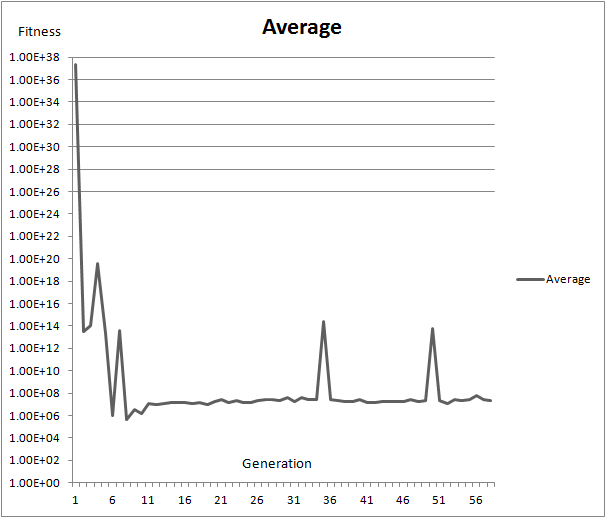
\includegraphics[]{Average}
\end{center}
\begin{center}
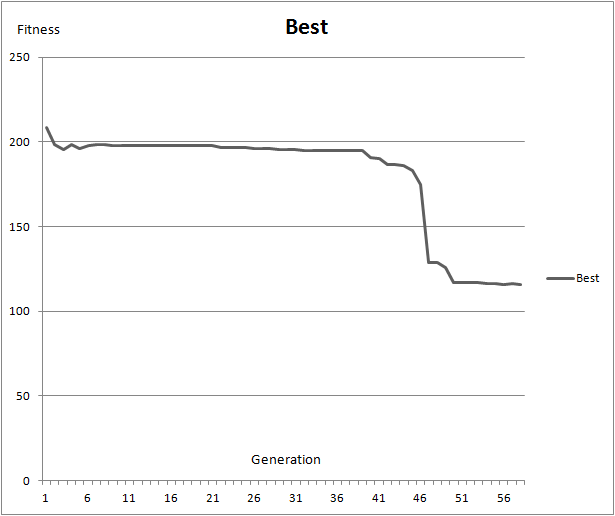
\includegraphics[]{Best}
\end{center}
\pagebreak

\paragraph{Graph} The following graph shows the data we were given and the data that my GP was able to produce. As you can see, the solution that I was able to produce through the GP was nothing close to what the actual data was producing. However compared to some of the worse fitness values, I am thoroughly impressed with the outcome considering how bad some of those graphs must look in comparison.

\begin{center}
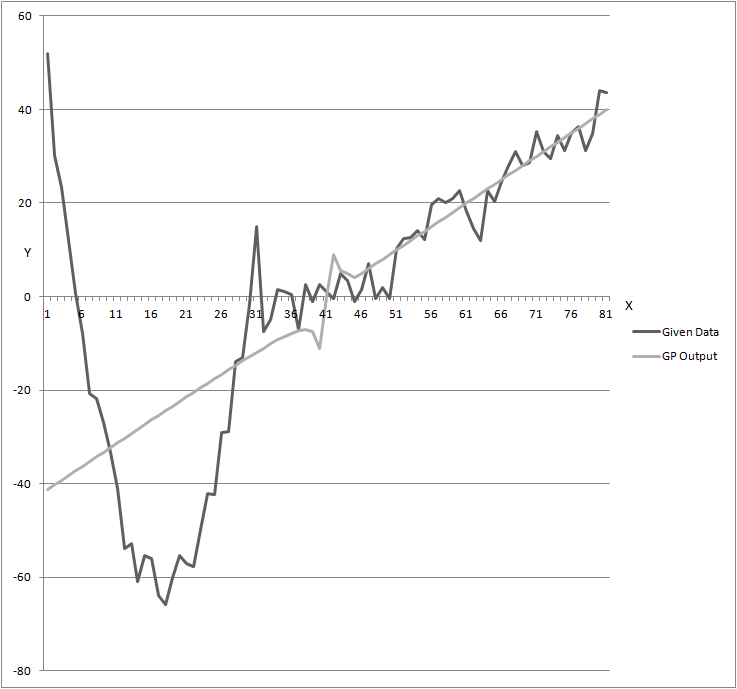
\includegraphics[scale = 0.75]{Graph}
\end{center}
\pagebreak

\section{Discussion}

\paragraph{Results} While I am happy with the GP being able to come up with a solution that is not just a straight line, some things arguably could have gone better and improved my GP substantially. The first thing is that even with deletion and protection on the tree, after roughly 60 generations the GP will fail because it has run out of memory. This is aggravating because with more time evolving it is possible that the GP would get a much better solution.

\paragraph{} Other than memory issues most everything else worked smoothly. Crossover was interesting as I had some debugging prints that would show how much of a tree was being swapped and interestingly enough it kept fairly small but when a big change to a tree happened, large jumps in fitness were almost always observed. These jumps were almost always for the worse but at least they showed that they were doing something.

\paragraph{Graphs} After multiple runs through the GP, it seems like my average fitness graph is a little abnormal in the fact that it stays somewhat stable. This is not the case for most of my other averages. After this section is a little bonus of some other graphs I got because I thought it was interesting that they all seem to be roughly the same graph with small variations at certain points which amazes me. If only I could get my program to evolve just a bit longer, I might be able to get to a point where a crossover or mutation takes two ok graphs and puts them together to make a great graph. Another observation is that more operators are definitely needed to get an almost perfect solution here. There is just no way to get some of the movements that the noise is producing without something that isn't a standard mathematical operator.

\section{Appendix A}

\begin{center}
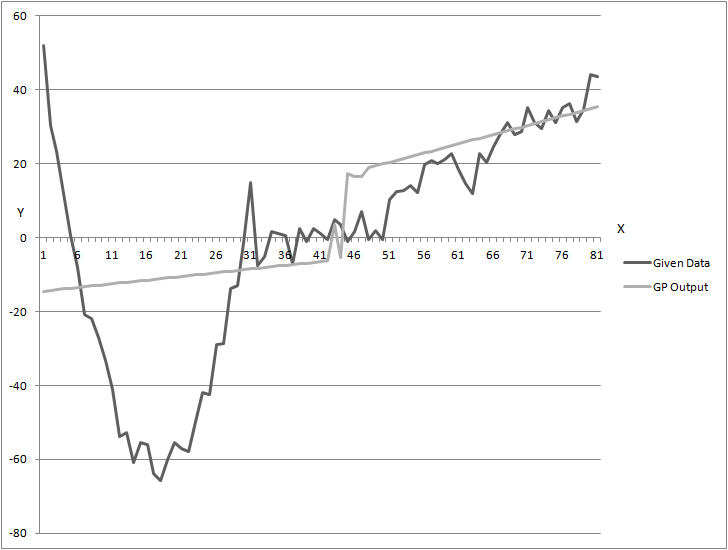
\includegraphics[scale = 0.75]{Graph2}
\end{center}
\pagebreak

\begin{center}
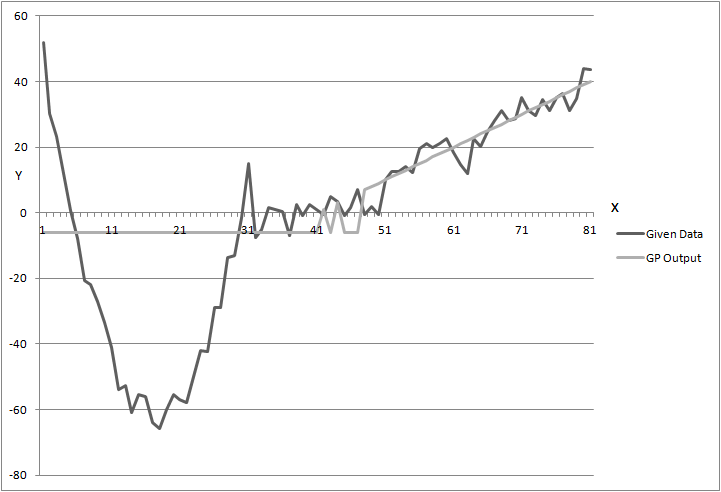
\includegraphics[scale = 0.8]{Graph3}
\end{center}
\pagebreak

\end{document}
